\documentclass[tikz,border=10pt]{standalone}
\usetikzlibrary{calc}
\begin{document}
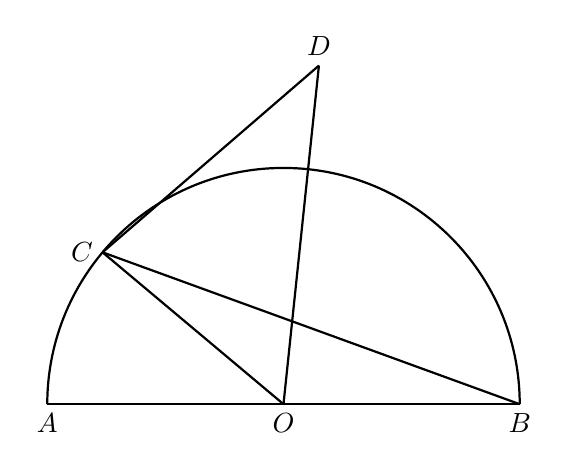
\begin{tikzpicture}
  \coordinate (O) at (0,0);
  \coordinate (A) at (-3,0);
  \coordinate (B) at (3,0);
  \coordinate (C) at (140:3);
  \coordinate (D) at (0.45,4.3);

  \draw[thick] (A) -- (B);
  \draw[thick] (A) arc (180:0:3);
  \draw[thick] (O) -- (D);
  \draw[thick] (C) -- (B);
  \draw[thick] (C) -- (O);
  \draw[thick] (C) -- (D);

  \node[below] at (A) {$A$};
  \node[below] at (O) {$O$};
  \node[below] at (B) {$B$};
  \node[left] at (C) {$C$};
  \node[above] at (D) {$D$};
\end{tikzpicture}
\end{document}
